\chapter{Umsetzung des Prototyps}
Nachdem in Kapitel \ref{sec:concept} die Konzeption der Anwendung vorgestellt wurde kann, kann nun die Umsetzung der Anwendungen erfolgen.

Zunächst wird dabei auf die Ausgangssituation aus dem vorangegangenem Projekt vorgestellt. Im Anschluss erfolgt eine Auflistung der verwendeten Technologien. Danach erfolgt die Vorstellung der Anwendungen, sowie die Herausforderungen und Probleme in der Umsetzung

\section{Ausgangssituation}
In der vorausgehenden Arbeit wurde ein Art \ac{MVP} der Spielidee umgesetzt welche aus 3 Hauptanwendungen bestand. Es gibt eine Unity-Anwendung, in welcher das Spielgeschehen des \say{Players} umgesetzt wurde. Das Spielgeschehen der \say{Watcher}-Anwendung wurde über eine Vue3-Webseite realisiert. Für die Kommunikation der beiden Anwendungen untereinander wurde auf der Basis eines \say{Express.js} Node-Servers ein WebSocket-Server entwickelt. Der Node-WebSocket-Server kommuniziert zusätzlich mit einer MongoDB Datenbank, in welcher die Fortschritte der einzelnen Sessions gespeichert werden.

Die Anwendungen des \say{Players} und des \say{Watchers} sind in dieser Konstellation jeweils Anzeigende und auf die Eingaben des Nutzers reagierende Komponenten im gesamten System. Sie geben eine Rückmeldung an den Server, der die Daten zur Laufzeit abspeichert und persistent in einer Datenbank speichern kann.

\subsection{Aufbau der Ausgangssituation}

Im Softwaredesign wird dabei von einem \ac{MVC} Design-Pattern gesprochen (vgl. \cite{GlossarWiki:Reenskaug:1979a}). 
Das Model definiert, welche Daten die App enthalten soll. Ändert sich der Zustand dieser Daten, informiert das Modell die einzelnen Views, damit die Ansicht der Daten entsprechend aktualisiert werden können. Außerdem wird manchmal auch der Controller über Änderungen informiert. Die View definiert wie die Daten angezeigt werden sollen. Der Controller verarbeitet die reinkommenden Änderungen aus den Views, die die Nutzer getätigt haben, und gibt diese an das Model oder die Views direkt weiter (vgl. \cite{noauthor_mvc_2023}); (vgl. Abbildung \ref{fig:mvc-diagramm}).

\begin{figure}[ht]
\centering
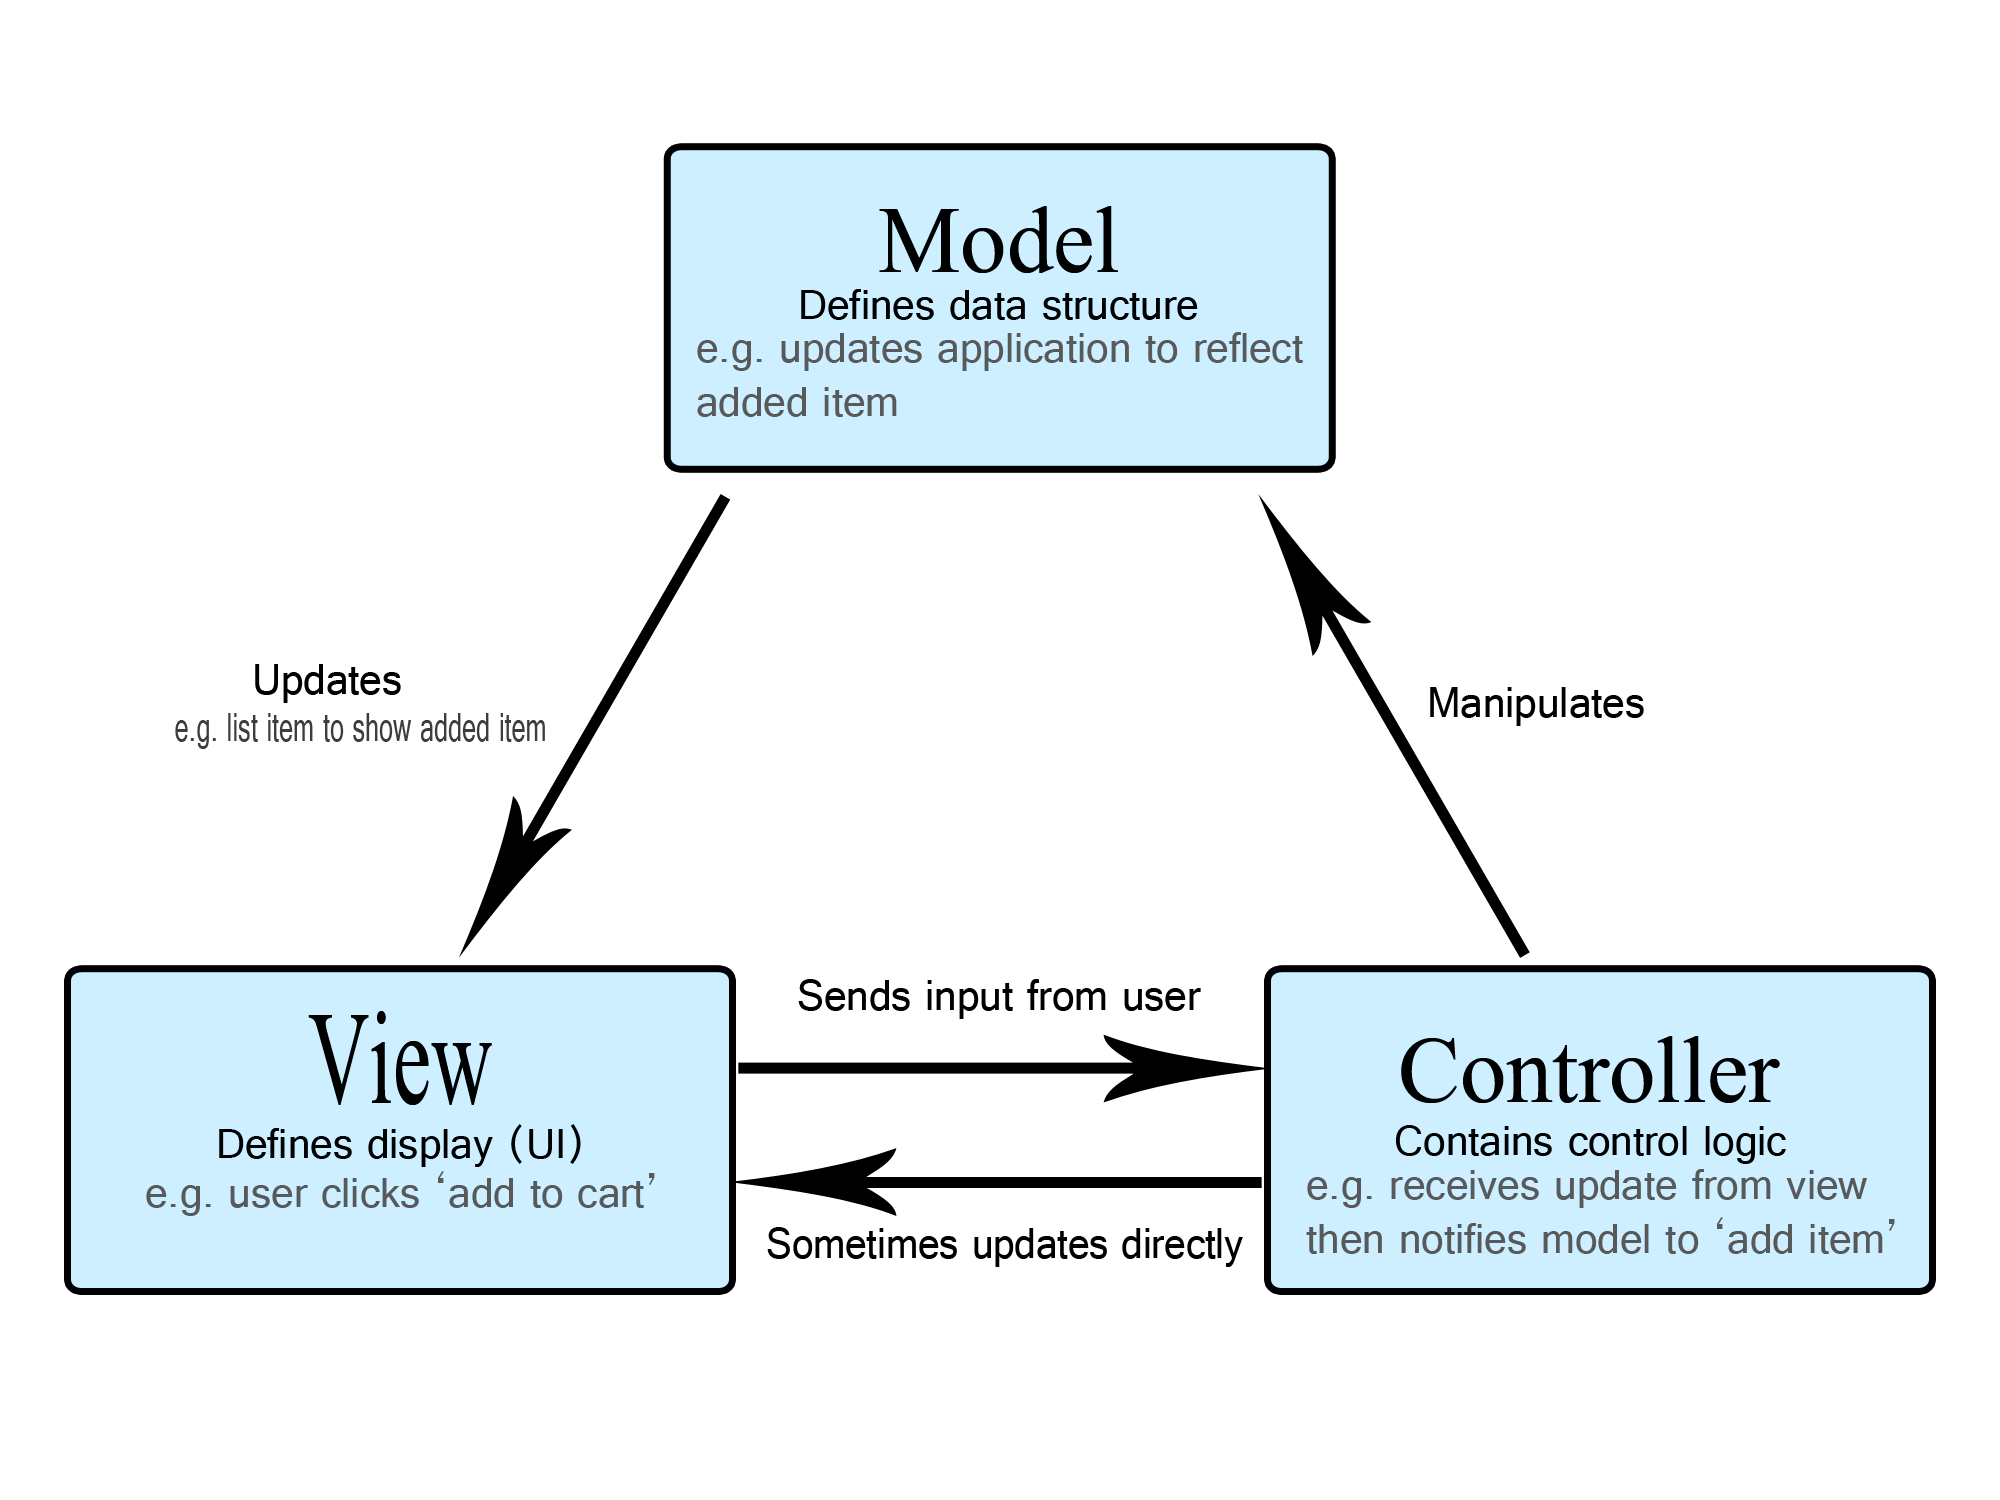
\includegraphics[width=1\linewidth]{content/pictures/mvc-architecture.png}
\caption{\ac{MVC} Beispiel-Diagramm \cite{noauthor_mvc_2023}}
\label{fig:mvc-diagramm}
\end{figure}

Die MongoDB Datenbank und Klassen innerhalb des WebSocket-Servers nehmen die Rolle des Model ein, die einzelnen WebSocket-Message Endpunkte übernehmen die Aufgaben des Controllers und die Anwendung des \say{Watchers} und des \say{Players} sind die Views der Architektur.

\subsection{Beitreten einer Session}

\begin{figure}[ht]
\centering
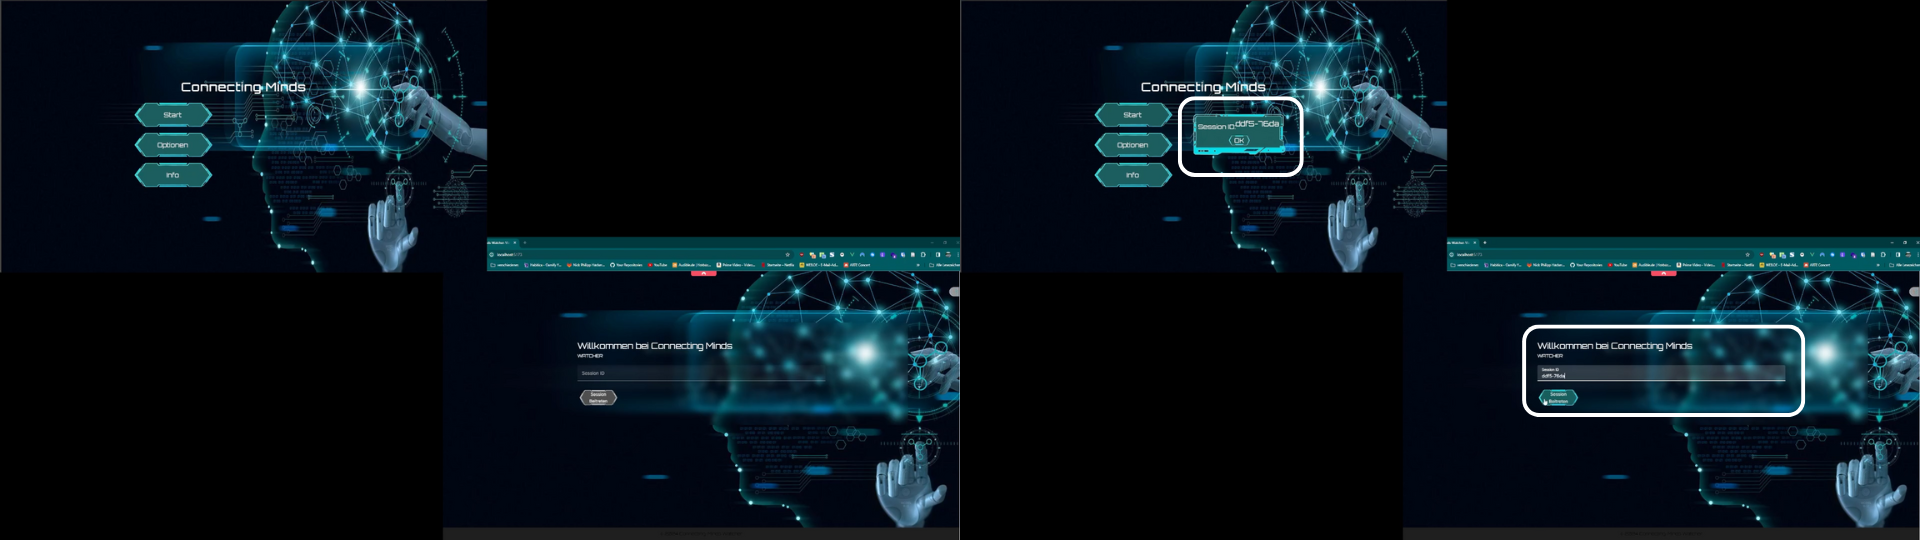
\includegraphics[width=1\linewidth]{content/pictures/Login_Login_by_ID.png}
\caption{Startbildschirme der Player und Watcher Anwendung (Quelle: eigene Darstellung)}
\label{fig:old-logins}
\end{figure}

Abbildung \ref{fig:old-logins} zeigt den bereits im alten Prototyp entwickelten Startbildschirm über welchen der Player eine neue Session starten (linkes Bild, links oben) und der Watcher dieser beitreten kann (linkes Bild, rechts unten). Sobald der Player eine Session erstellt hat, erhält er vom WebSocket-Server eine Rückmeldung mit der erstellten Session-ID (rechtes Bild, links oben) welches er dem Watcher mitteilen muss, damit dieser ihr beitreten kann (rechts Bild, rechts unten).

\subsection{Einführung in die Anwendungen}

\begin{figure}[ht]
\centering
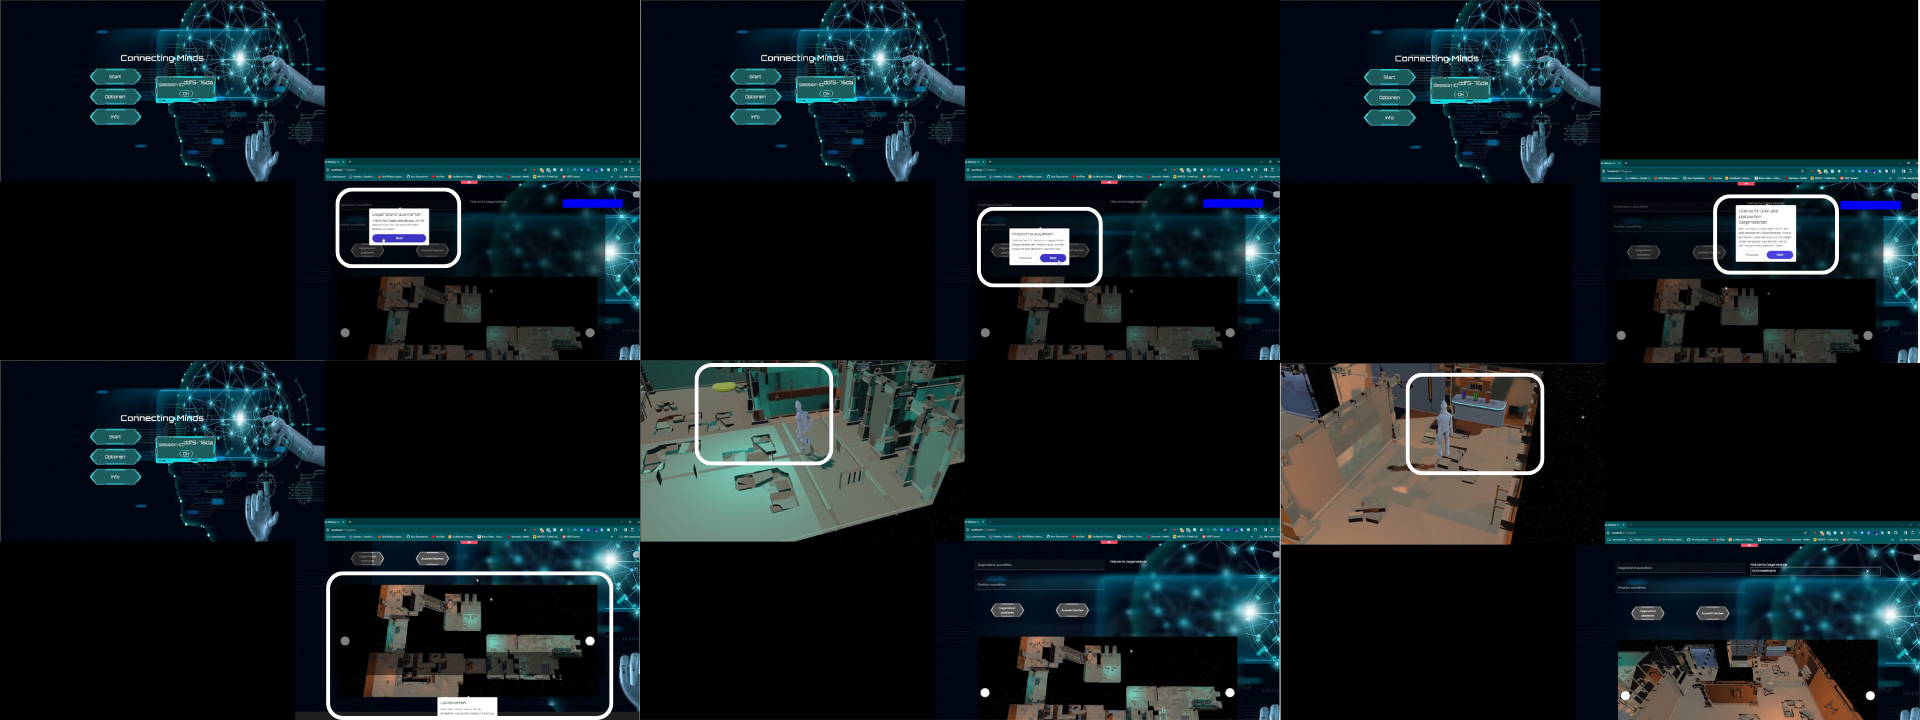
\includegraphics[width=1\linewidth]{content/pictures/Introduction.png}
\caption{Einführung in die Anwendung des Players und Watchers (Quelle: eigene Darstellung)}
\label{fig:old-logins}
\end{figure}

\subsection{Lösen von Rätseln}

\subsection{Freischalten von Gegenständen und Positionen}

\subsection{Aspekte zum Überarbeiten}

\section{Verwendete Technologien}



\section{Aufbau des Prototyps}



\section{Herausforderungen in der Umsetzung}
% hier kommt das placing also die positionen in der spielwelt

% dann drauf bezogen das mit den slots, dass die ne position haben später auch fürs setzen wichtig
% das mit den collidern, was man auch anders umsetzen kann noch, das noch erwähnen






% bei umsetzung müssen die 3d und ar anwendung vorgestellt werden vom watcher
% hier muss ein bezg auf das paper mit den steuerungen für touch erwähnt werden


% die anwendung vom playewr

\section{Probleme in der Umsetzung}